%% myFigures.tex
% A common file to store all figure definitions
%
% In preparing your thesis, one of the first things you should do is
% organize your figures.  Then, one of the last things you'll do is
% reorder your figures so they display where you want them to in the
% text.  Organizing figure definitions in a common files helps:
%
%   1. Write new figures using earlier examples.
%
%   2.  Isolate code and minimize the risk of introducing bugs in the
%   final editing process.  Trust me, moving around just one line of
%   code is easier.
%
%   3.  Reuse figures in other papers.  <=== the best reason!
%
% Note command names can not include numbers and special characters.
%
% To make the file more searchable, use naming conventions that map
% the graphics filename labSetup.jpg to the command name \figlabSetup to the
% figure label fig:labSetup.
% 

\newcommand{\figMpduFormat}{
	\begin{figure}[H]
		\begin{center}
			\makebox[\textwidth][c]{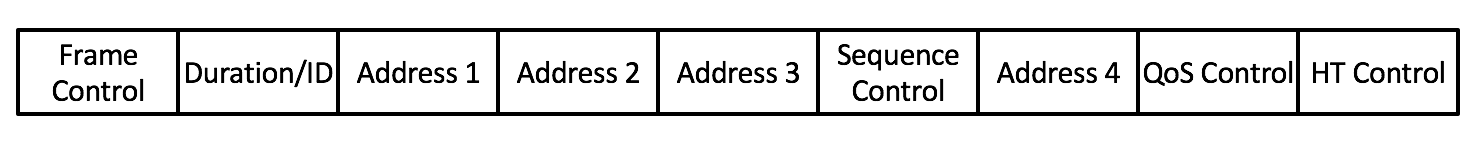
\includegraphics[width=\linewidth]{macHeader}}
			\caption{\ac{MPDU} format when using \ac{WPA}-2 \cite{802.11}}
			\label{fig:MpduFormat}
		\end{center}
		\vspace{-0.2 in}
	\end{figure}
}

\newcommand{\figMacHeader}{
	\begin{figure}[H]
		\begin{center}
			\makebox[\textwidth][c]{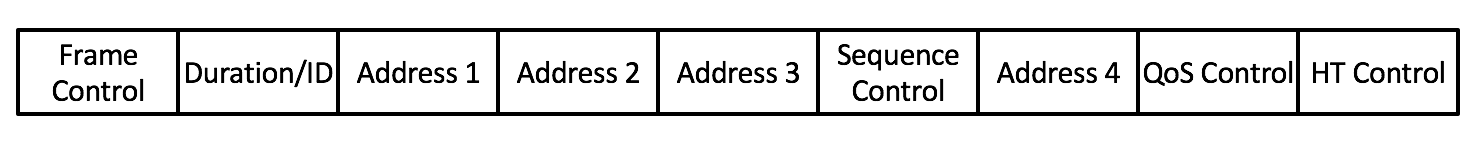
\includegraphics[width=\linewidth]{macHeader}}
			\caption{\ac{MAC} Header Frame Format \cite{802.11}}
			\label{fig:MacHeader}
		\end{center}
		\vspace{-0.2 in}
	\end{figure}
}

\newcommand{\figArchitecture}{\begin{figure}[H]
	\begin{center}
		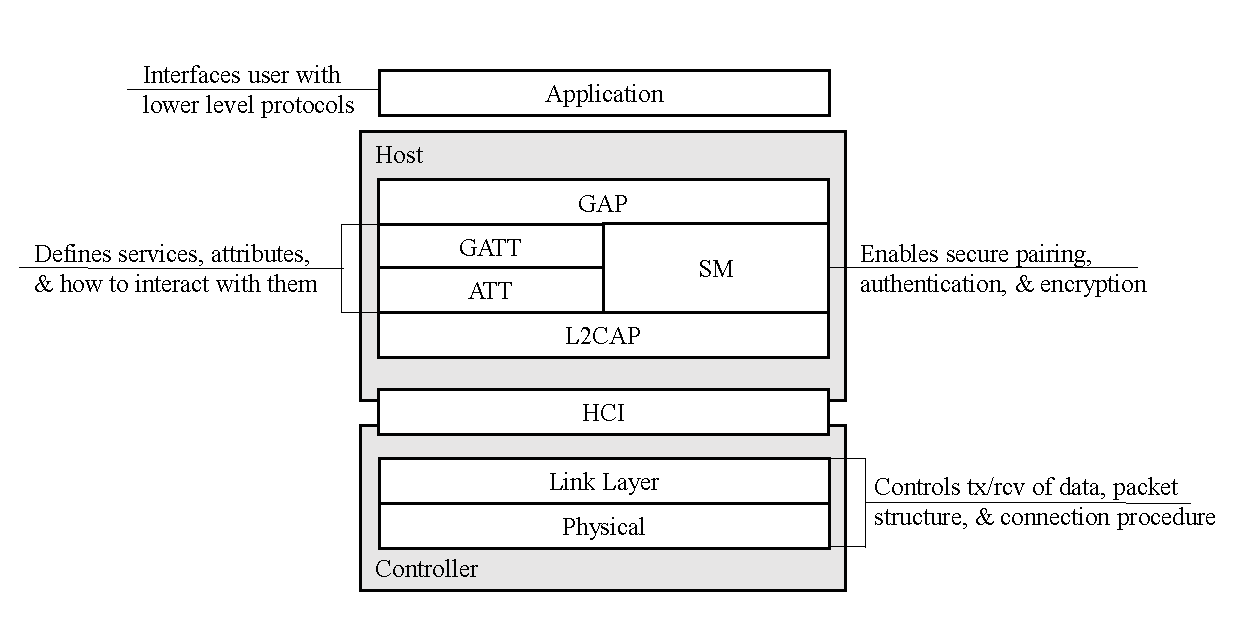
\includegraphics[width=4in]{architecture}
		\caption{The Bluetooth Low Energy Architecture}
		\label{fig:Architecture}
	\end{center}
	\vspace{-0.2 in}
\end{figure}
}

\newcommand{\figConnection}{\begin{figure}[H]
	\begin{center}
		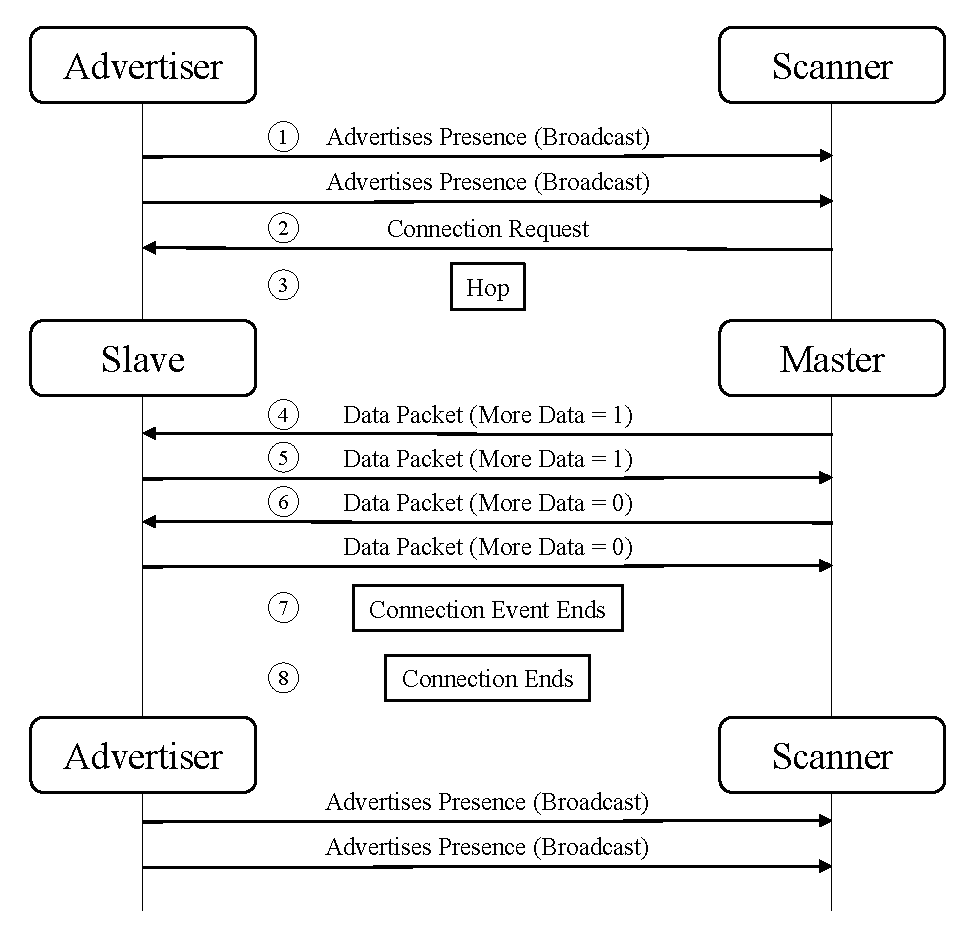
\includegraphics[width=4in]{connectionProcess}
		\caption{The \ac{BLE} Connection Process}
		\label{fig:Connection}
	\end{center}
	\vspace{-0.2 in}
\end{figure}
}

\newcommand{\figScanning}{\begin{figure}[H]
		\begin{center}
			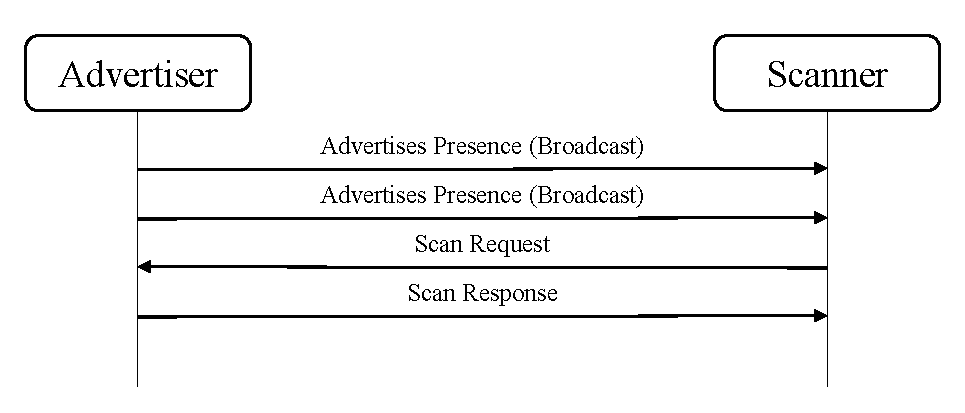
\includegraphics[width=4in]{activeScanning}
			\caption{Active Scanning Process}
			\label{fig:Scanning}
		\end{center}
		\vspace{-0.2 in}
	\end{figure}
}

\newcommand{\figChannel}{
	\begin{figure}[H]
		\begin{center}
			\includegraphics[width=5in]{channelMap}
			\caption{Bluetooth Low Energy channel mapping; darker channels represent advertisement channels}
			\label{fig:Channel}
		\end{center}
		\vspace{-0.2 in}
	\end{figure}
}

\newcommand{\figAccessPoint}{
	\begin{figure}[H]
		\begin{center}
			\makebox[\textwidth][c]{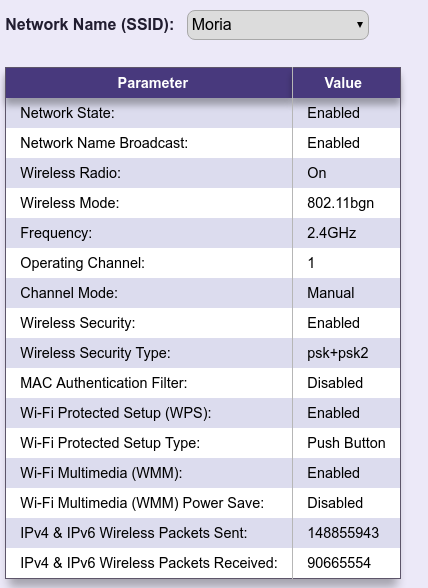
\includegraphics[width=2.5in]{accessPoint}}
			\caption{Prancing Pony Access Point Settings}
			\label{fig:AccessPoint}
		\end{center}
		\vspace{-0.2 in}
	\end{figure}
}

\newcommand{\figSystemDiagram}{
	\begin{figure}[h!]
		\begin{center}
			\centering
			\makebox[\textwidth][c]{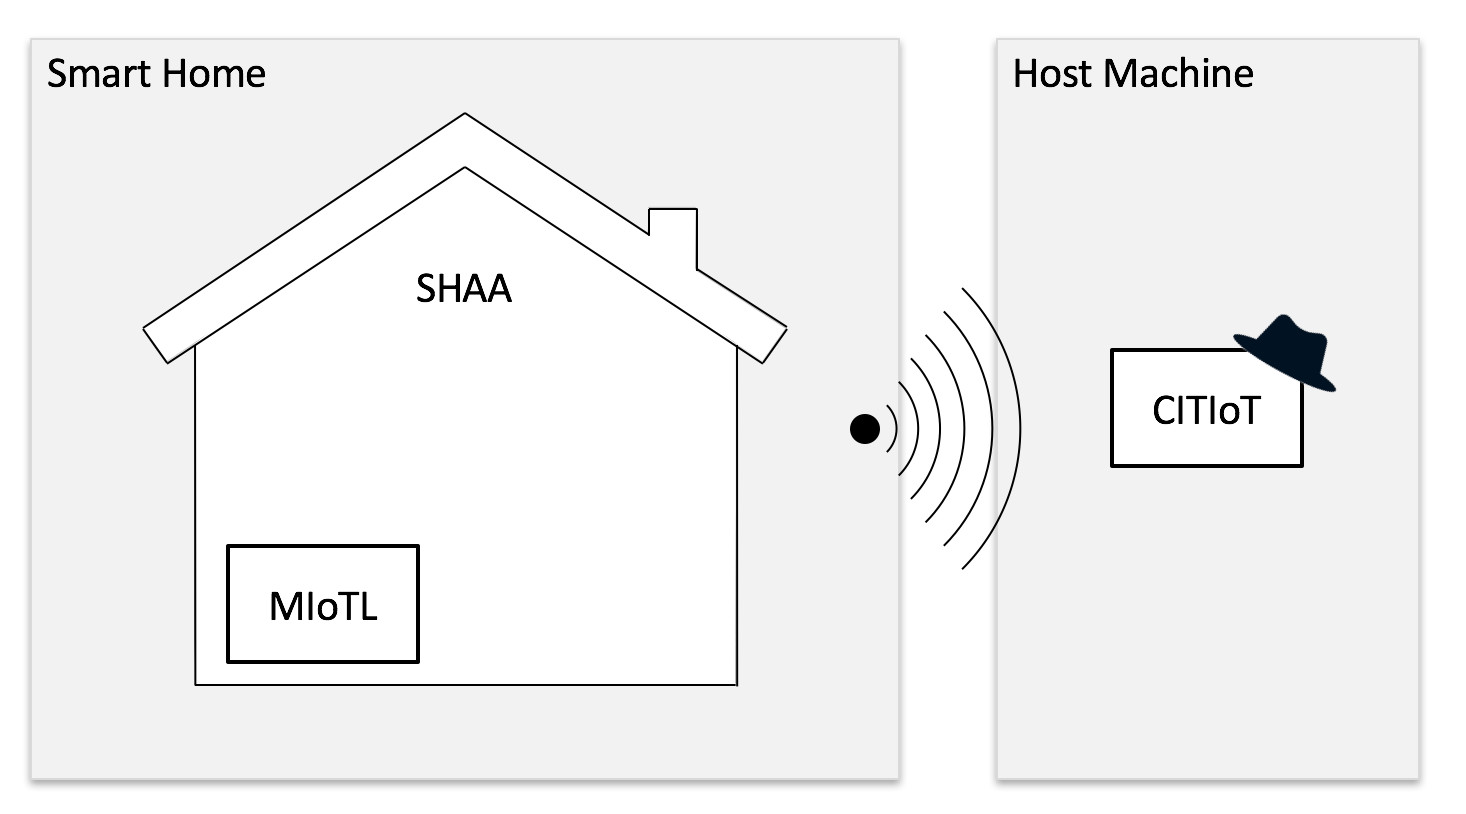
\includegraphics[width=4in]{systemDiagram}}
			\caption{Overall system diagram}
			\label{fig:SystemDiagram}
		\end{center}
		\vspace{-0.2 in}
	\end{figure}
}

\newcommand{\figShaaDiagram}{
	\begin{figure*}[h!]
		\begin{center}
			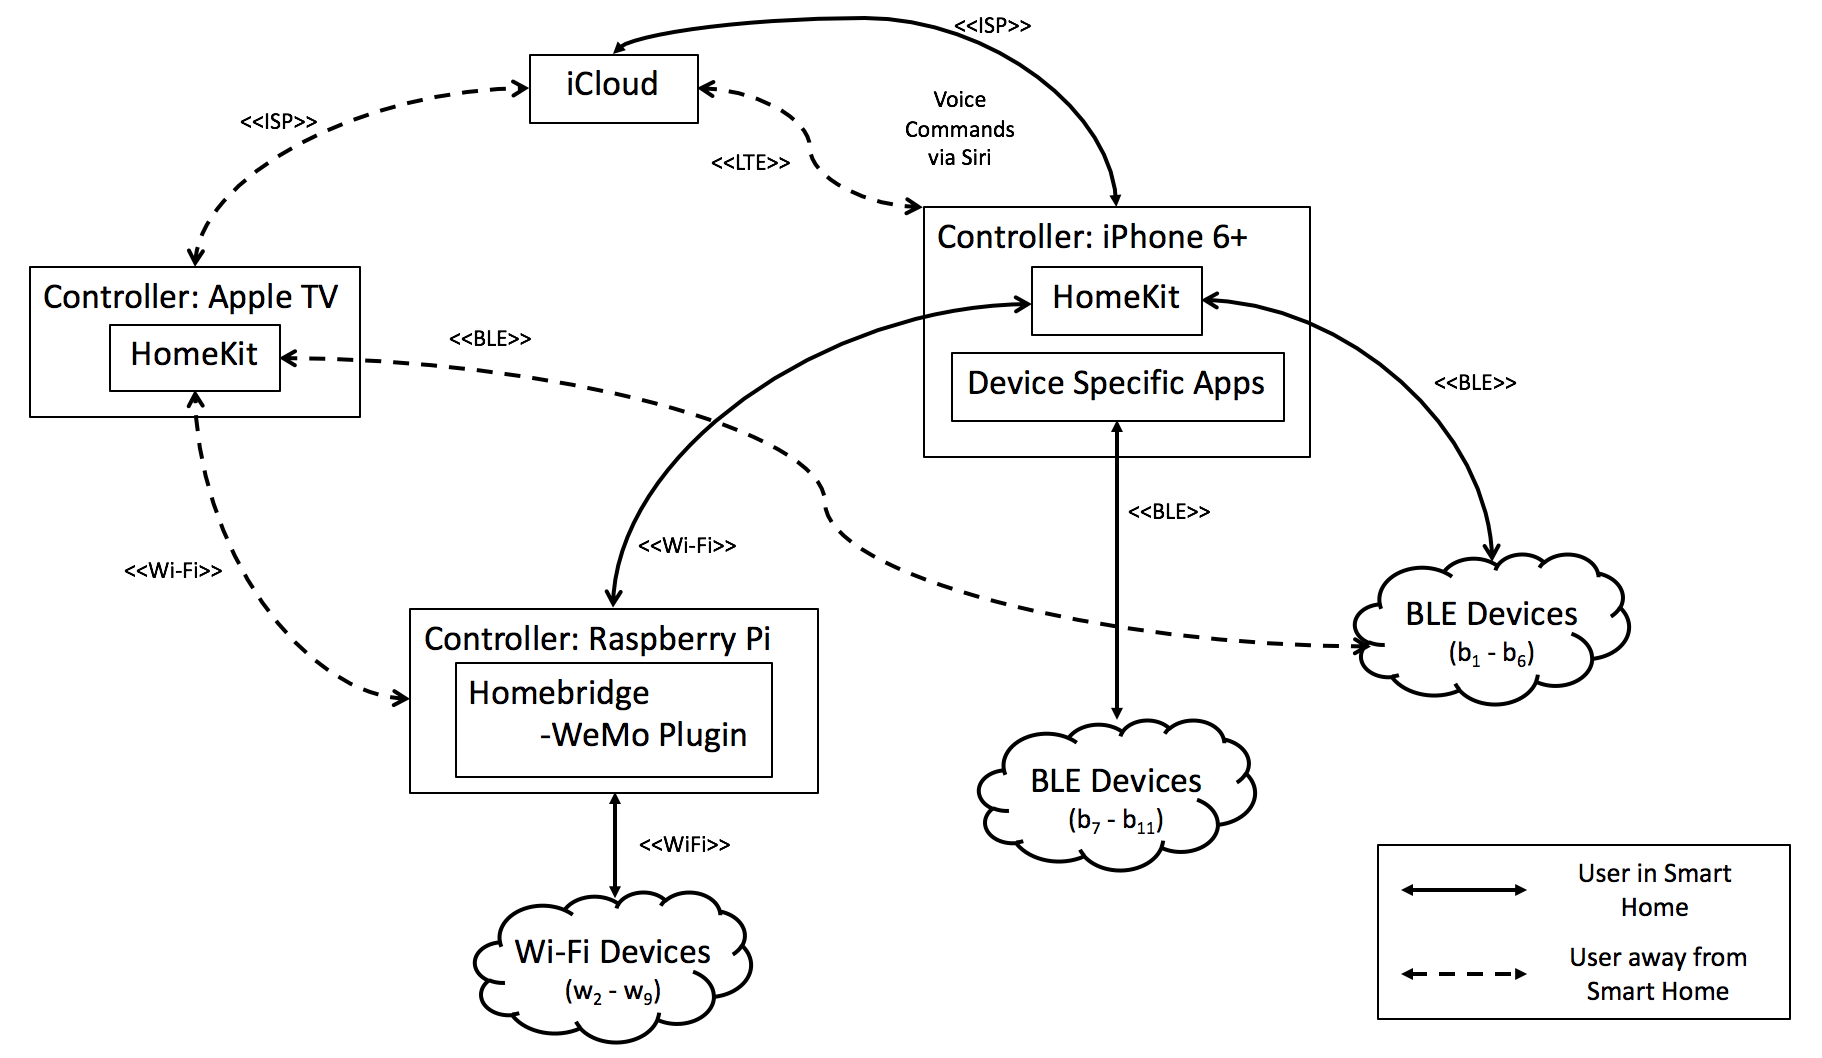
\includegraphics[width=\linewidth]{shaaDiagram}
			\caption{Diagram of SHAA components}
			\label{fig:ShaaDiagram}
		\end{center}
		\vspace{-0.2 in}
	\end{figure*}
}

\newcommand{\figCitiotDiagram}{
	\begin{figure*}[h!]
		\begin{center}
			\makebox[\textwidth][c]{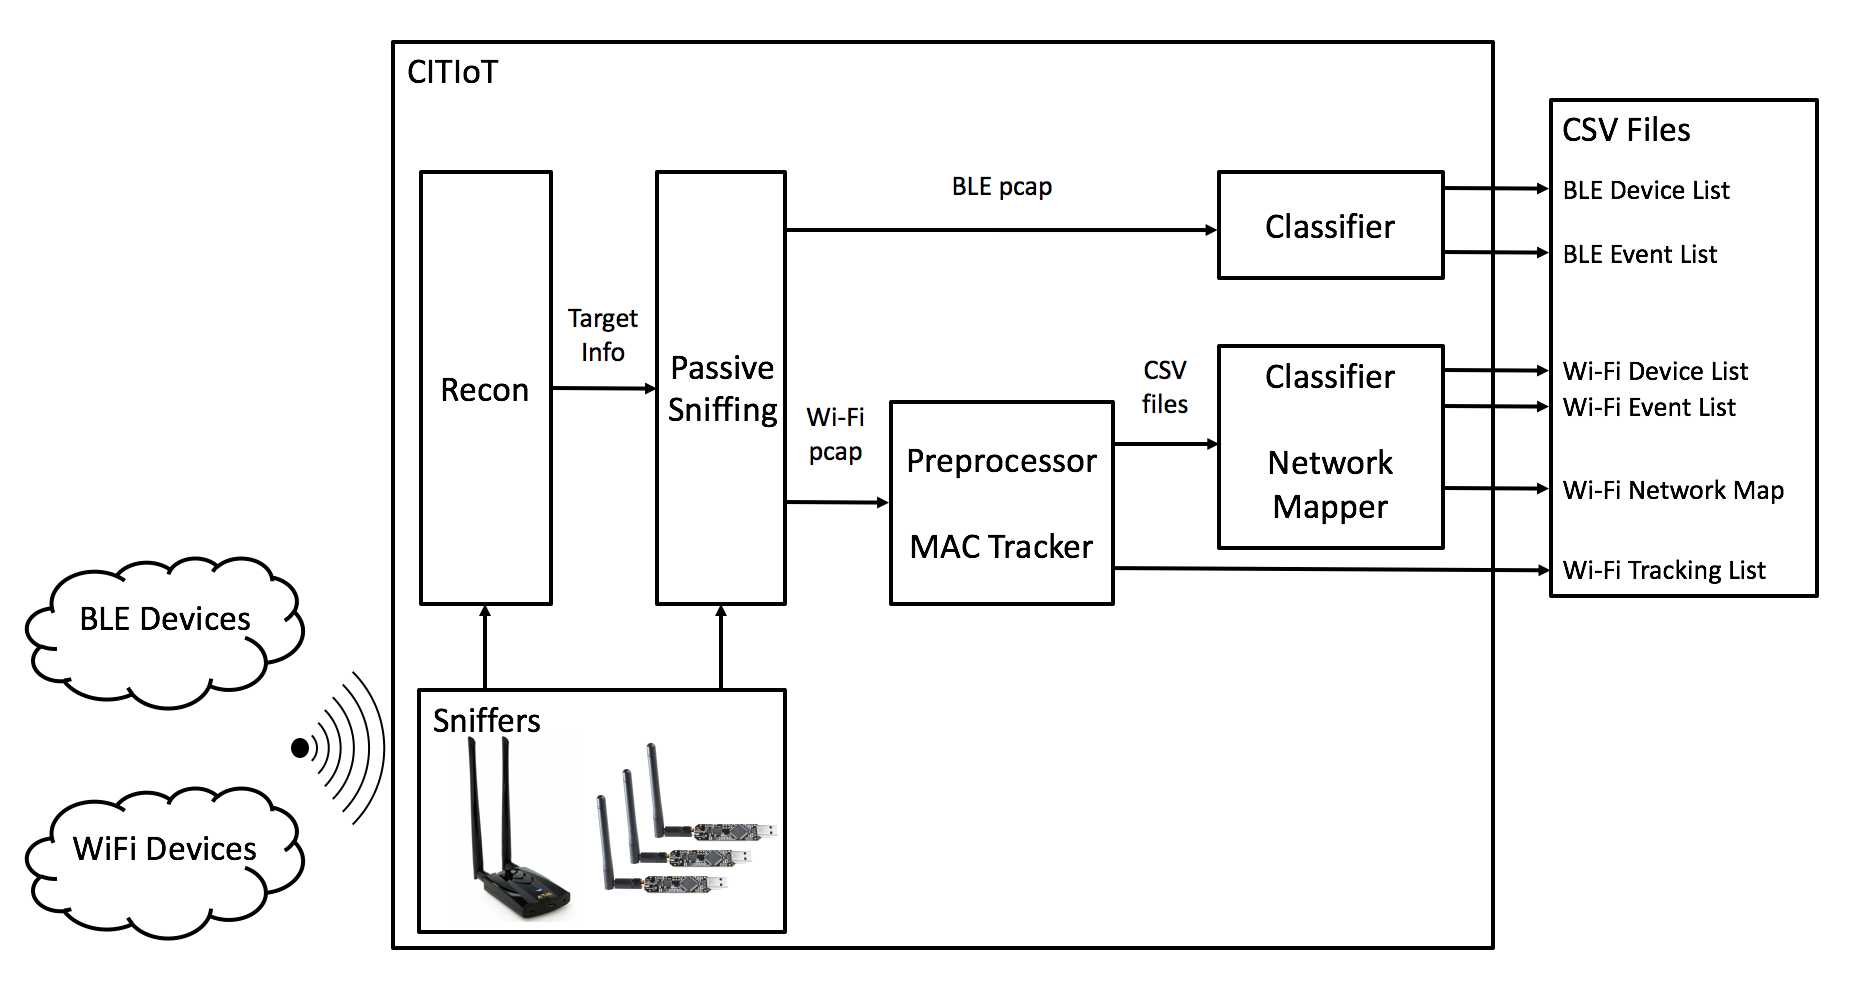
\includegraphics[width=\linewidth]{citiotDiagram}}
			\caption{Diagram of CITIoT tool components and interactions}
			\label{fig:CitiotDiagram}
		\end{center}
		\vspace{-0.2 in}
	\end{figure*}
}

\newcommand{\figReconScan}{
	\begin{figure*}[h!]
		\begin{center}
			\makebox[\textwidth][c]{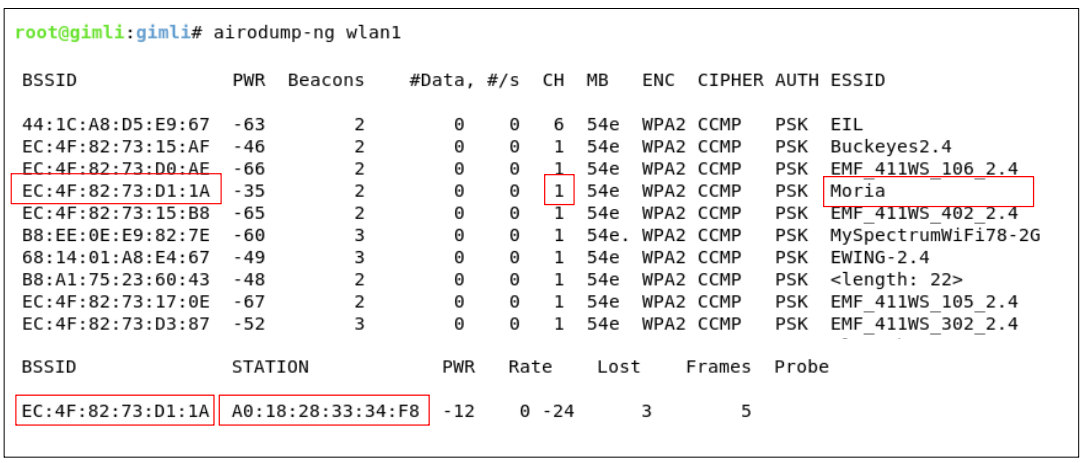
\includegraphics[width=\linewidth]{reconScan}}
			\caption{Command and results to accomplish a scan of Wi-Fi devices and associated \ac{AP}s}
			\label{fig:ReconScan}
		\end{center}
		\vspace{-0.2 in}
	\end{figure*}
}

\newcommand{\figScanDevices}{
	\begin{figure}[H]
		\begin{center}
			\makebox[\textwidth][c]{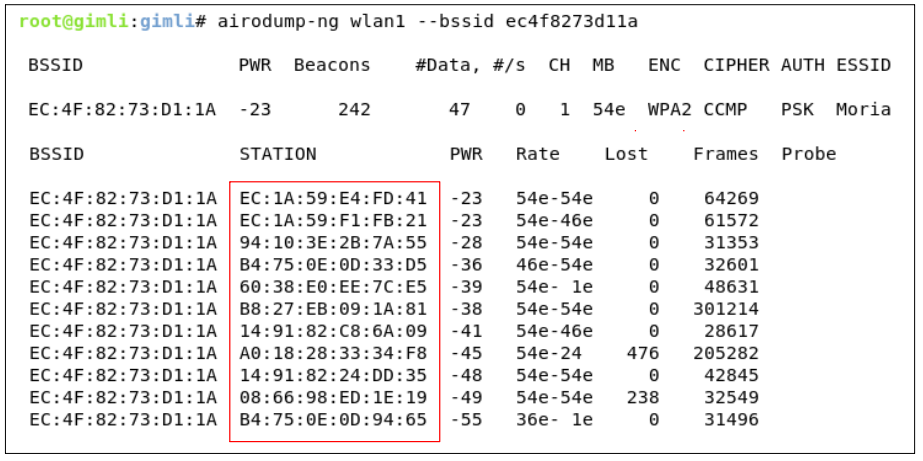
\includegraphics[width=\linewidth]{scanDevices}}
			\caption{Command and results to scan for devices connected to the target \ac{AP}}
			\label{fig:ScanDevices}
		\end{center}
		\vspace{-0.2 in}
	\end{figure}
}

\newcommand{\figOuiLookup}{
	\begin{figure}[H]
		\begin{center}
			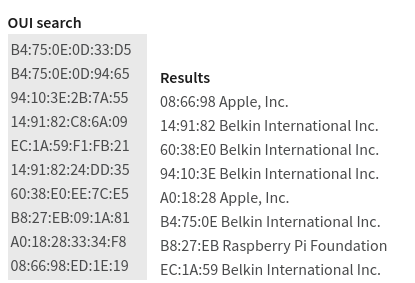
\includegraphics[width=3in]{ouiLookup}
			\caption{Wi-Fi MAC OUI search and results}
			\label{fig:OuiLookup}
		\end{center}
		\vspace{-0.2 in}
	\end{figure}
}

\newcommand{\figBleDeviceScan}{
	\begin{figure}[H]
		\begin{center}
			\makebox[\textwidth][c]{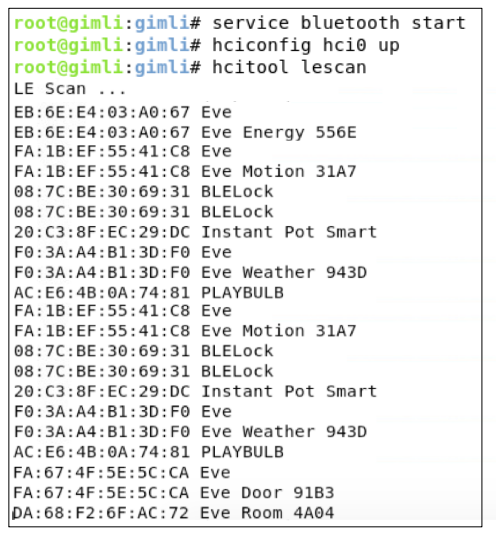
\includegraphics[width=3.5in]{bleDeviceScan}}
			\caption{Command and results to scan for \ac{BLE} devices within the smart home}
			\label{fig:BleDeviceScan}
		\end{center}
		\vspace{-0.2 in}
	\end{figure}
}

\newcommand{\figMonitorMode}{
	\begin{figure}[H]
		\begin{center}
			\makebox[\textwidth][c]{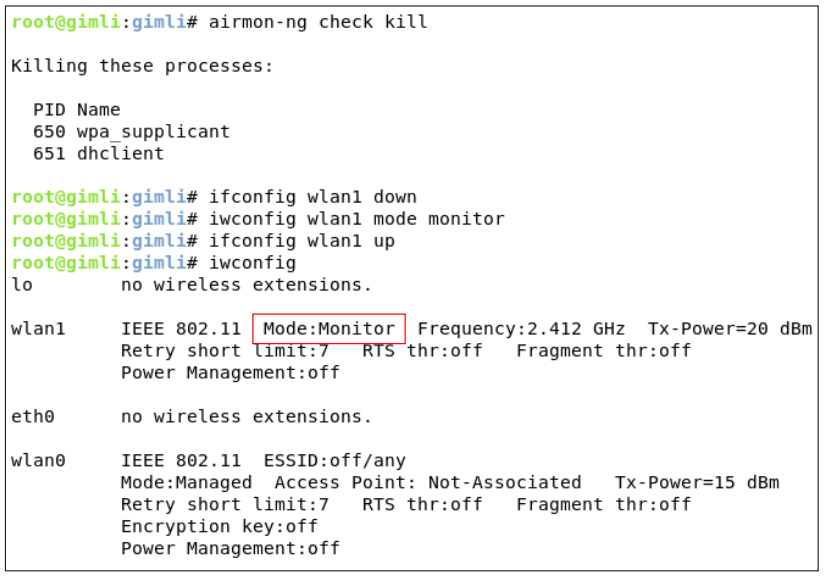
\includegraphics[width=\linewidth]{monitorMode}}
			\caption{Commands used to set Wi-Fi interface to monitor mode}
			\label{fig:MonitorMode}
		\end{center}
		\vspace{-0.2 in}
	\end{figure}
}

\newcommand{\figWifiCaptCmd}{
	\begin{figure}[H]
		\begin{center}
			\makebox[\textwidth][c]{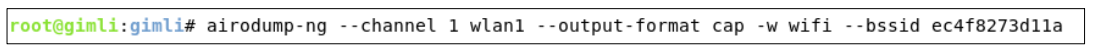
\includegraphics[height=.75cm]{wifiCaptCmd}}
			\caption{Command and options used to capture Wi-Fi traffic}
			\label{fig:WifiCaptCmd}
		\end{center}
		\vspace{-0.2 in}
	\end{figure}
}

\newcommand{\figBleCaptCmd}{
	\begin{figure}[H]
		\begin{center}
			\makebox[\textwidth][c]{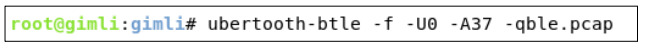
\includegraphics[height=.75cm]{bleCaptCmd}}
			\caption{Example command and options used to capture \ac{BLE} traffic}
			\label{fig:BleCaptCmd}
		\end{center}
		\vspace{-0.2 in}
	\end{figure}
}

\newcommand{\figCorruptTimePacket}{
	\begin{figure}[H]
		\begin{center}
			\makebox[\textwidth][c]{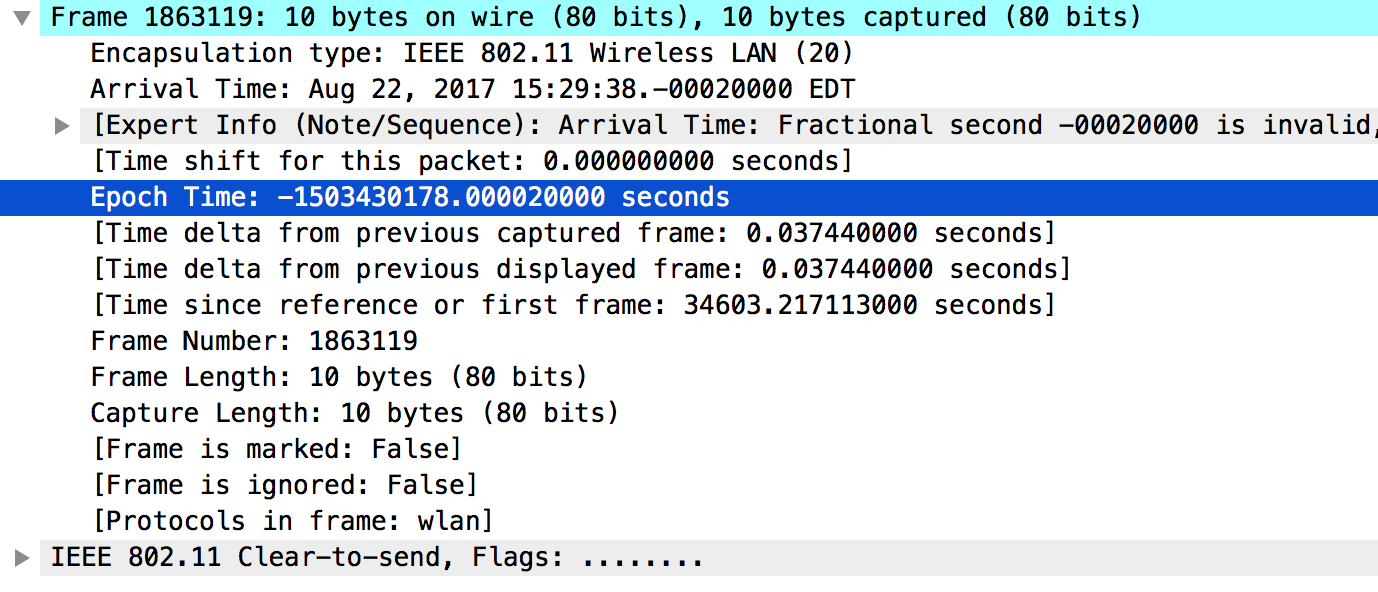
\includegraphics[width=\linewidth]{corruptTimePacket}}
			\caption{Encrypted packet used in \ac{MAC} tracker showing corrupted timestamp}
			\label{fig:CorruptTimePacket}
		\end{center}
		\vspace{-0.2 in}
	\end{figure}
}

\newcommand{\figWrongFrameNumber}{
	\begin{figure}[H]
		\begin{center}
			\makebox[\textwidth][c]{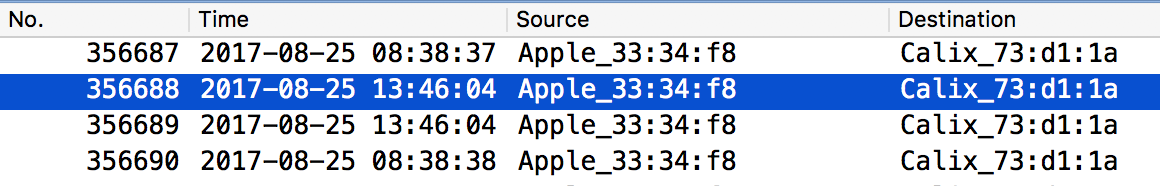
\includegraphics[width=\linewidth]{wrongFrameNumber}}
			\caption{Encrypted packets used in \ac{MAC} tracker showing sequential frame numbers but wrong times}
			\label{fig:WrongFrameNumber}
		\end{center}
		\vspace{-0.2 in}
	\end{figure}
}

\newcommand{\figTrainingToDevice}{
	\begin{figure}[H]
		\centering
		\begin{subfigure}{.485\textwidth}
			\centering
			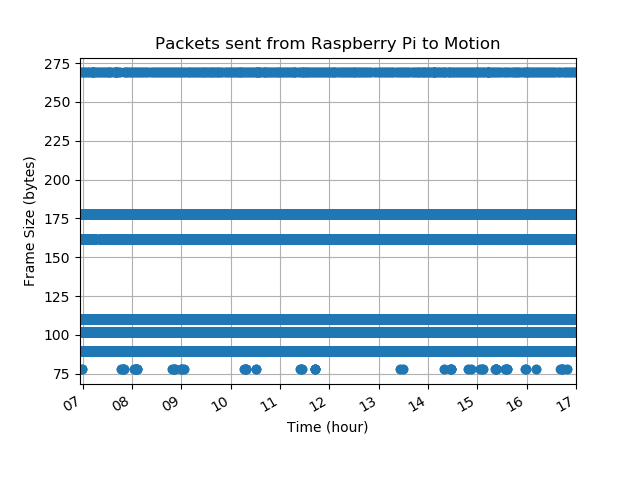
\includegraphics[width=\linewidth]{trngToMotion}
			\caption{}
		\end{subfigure}%
		\begin{subfigure}{.485\textwidth}
			\centering
			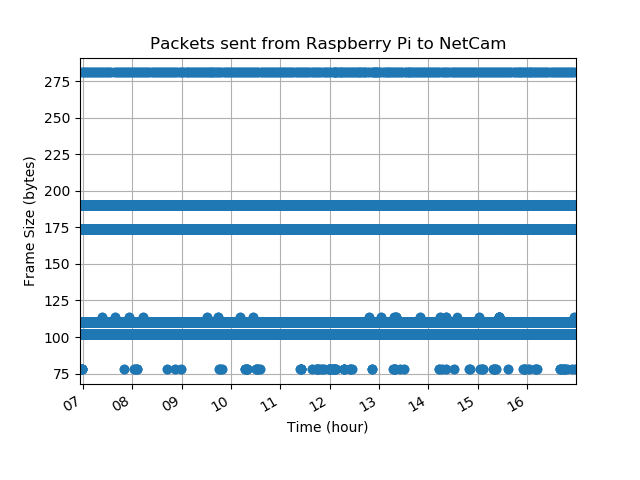
\includegraphics[width=\linewidth]{trngToNetcam}
			\caption{}
		\end{subfigure}
		\begin{subfigure}{.485\textwidth}
			\centering
			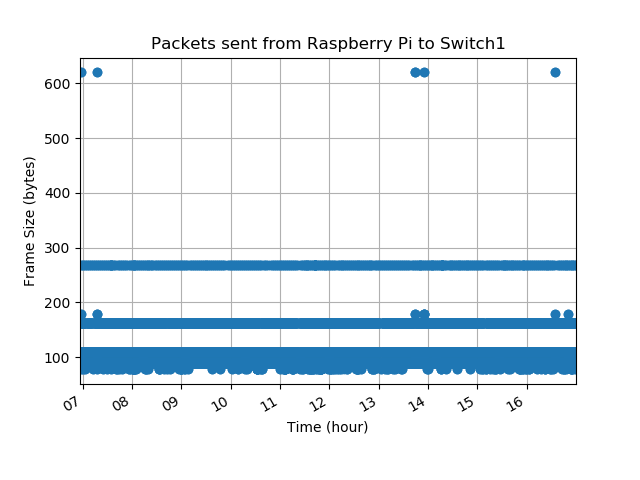
\includegraphics[width=\linewidth]{trngToSwitch1}
			\caption{}
		\end{subfigure}%
		\begin{subfigure}{.485\textwidth}
			\centering
			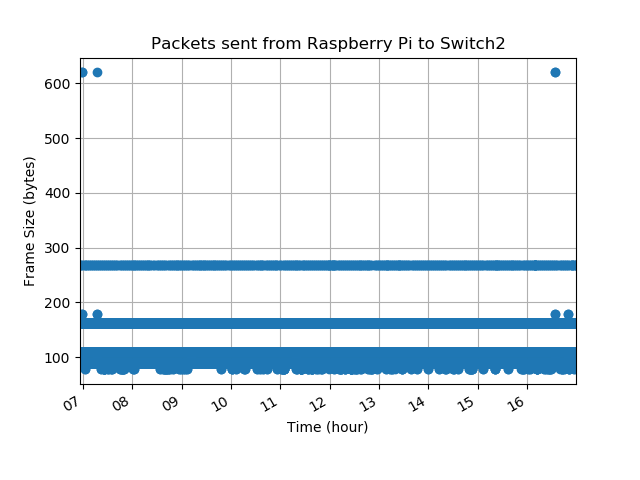
\includegraphics[width=\linewidth]{trngToSwitch2}
			\caption{}
		\end{subfigure}
		\begin{subfigure}{.485\textwidth}
			\centering
			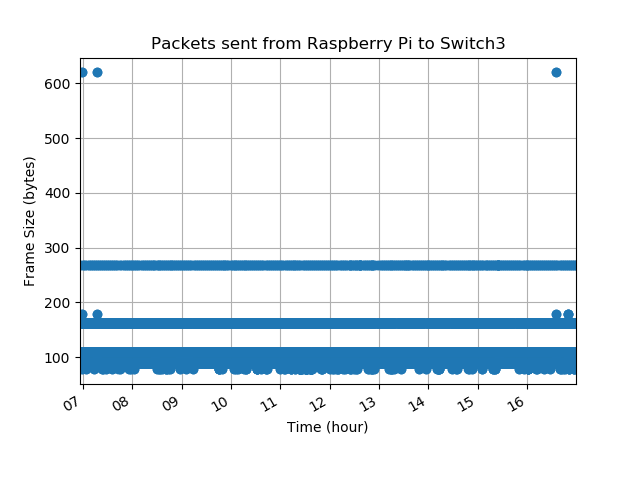
\includegraphics[width=\linewidth]{trngToSwitch3}
			\caption{}
		\end{subfigure}%
		\begin{subfigure}{.485\textwidth}
			\centering
			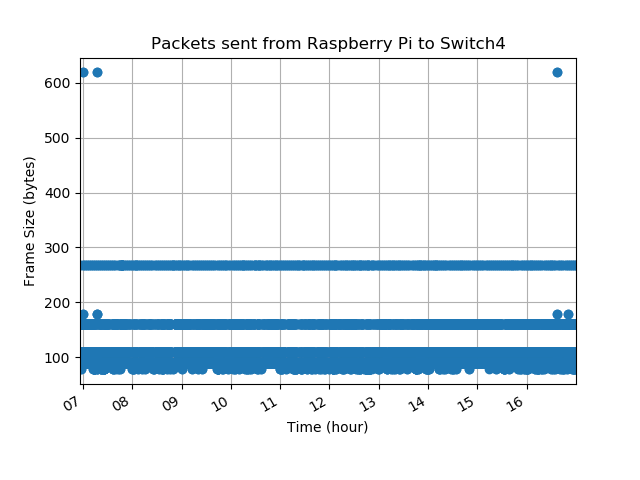
\includegraphics[width=\linewidth]{trngToSwitch4}
			\caption{}
		\end{subfigure}
		\begin{subfigure}{.485\textwidth}
			\centering
			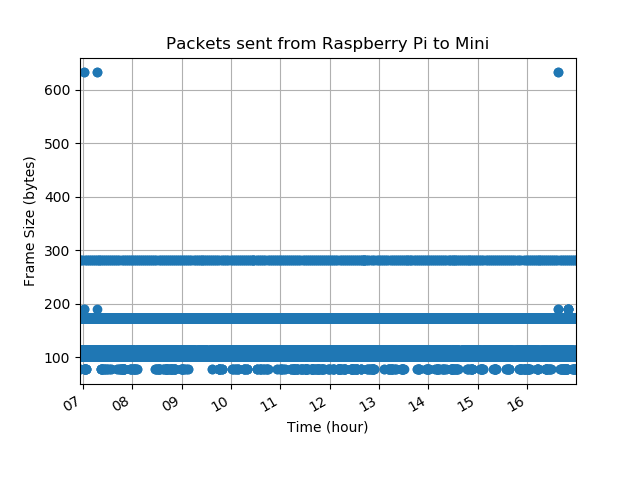
\includegraphics[width=\linewidth]{trngToMini}
			\caption{}
		\end{subfigure}%
		\begin{subfigure}{.485\textwidth}
			\centering
			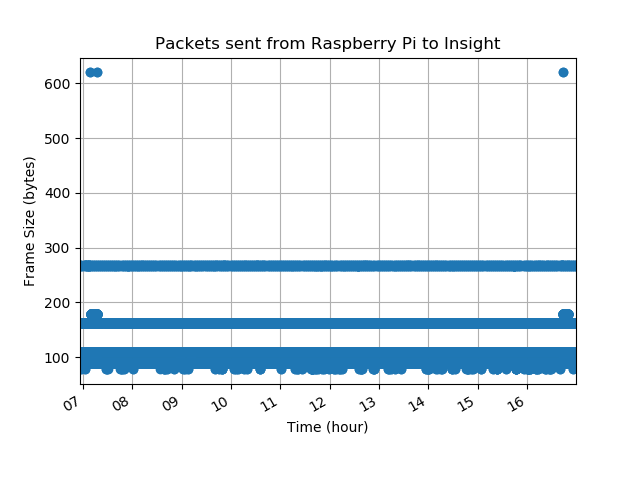
\includegraphics[width=\linewidth]{trngToInsight}
			\caption{}
		\end{subfigure}
		\caption{Training plots of packets sent from raspberry pi to device}
		\label{fig:TrainingToDevice}
	\end{figure}
}

\newcommand{\figTrainingFromDevice}{
	\begin{figure}[H]
		\centering
		\begin{subfigure}{.485\textwidth}
			\centering
			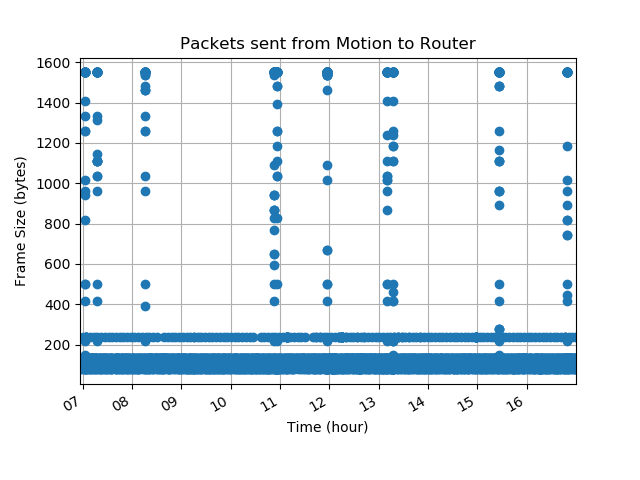
\includegraphics[width=\linewidth]{trngFromMotion}
			\caption{}
		\end{subfigure}%
		\begin{subfigure}{.485\textwidth}
			\centering
			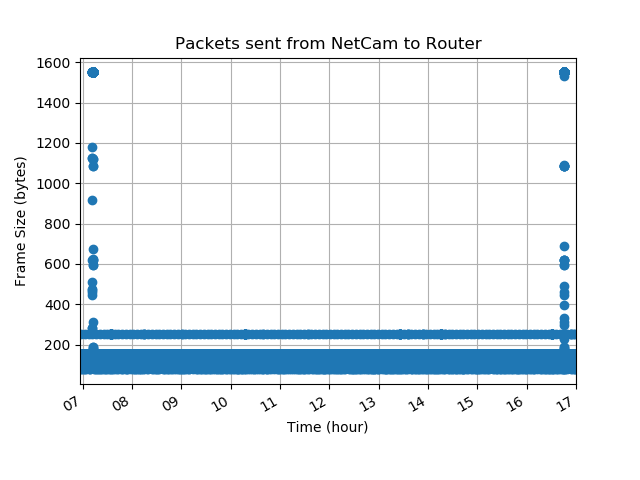
\includegraphics[width=\linewidth]{trngFromNetcam}
			\caption{}
		\end{subfigure}
		\begin{subfigure}{.485\textwidth}
			\centering
			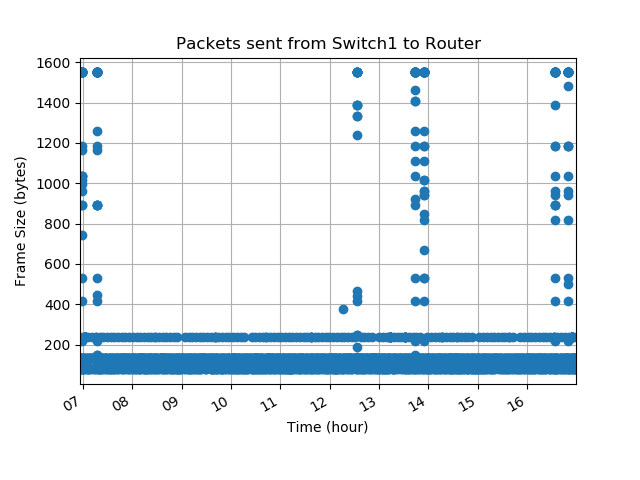
\includegraphics[width=\linewidth]{trngFromSwitch1}
			\caption{}
		\end{subfigure}%
		\begin{subfigure}{.485\textwidth}
			\centering
			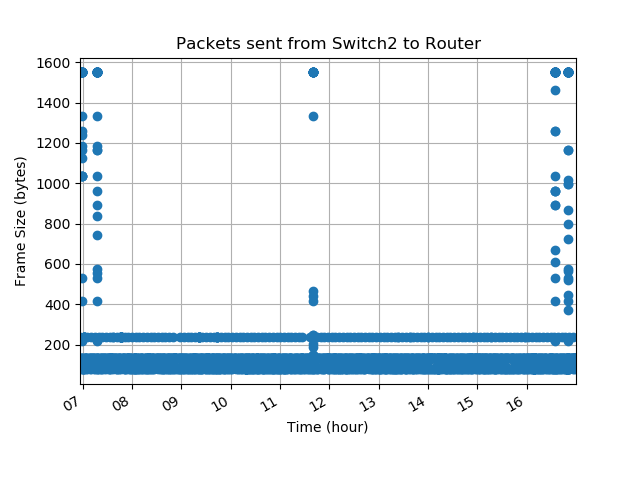
\includegraphics[width=\linewidth]{trngFromSwitch2}
			\caption{}
		\end{subfigure}
		\begin{subfigure}{.485\textwidth}
			\centering
			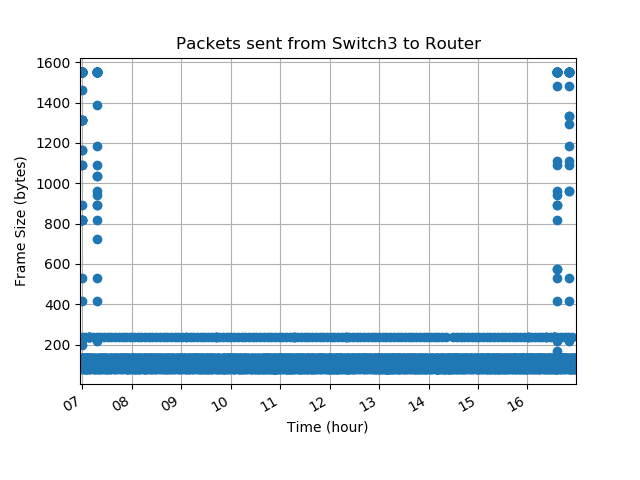
\includegraphics[width=\linewidth]{trngFromSwitch3}
			\caption{}
		\end{subfigure}%
		\begin{subfigure}{.485\textwidth}
			\centering
			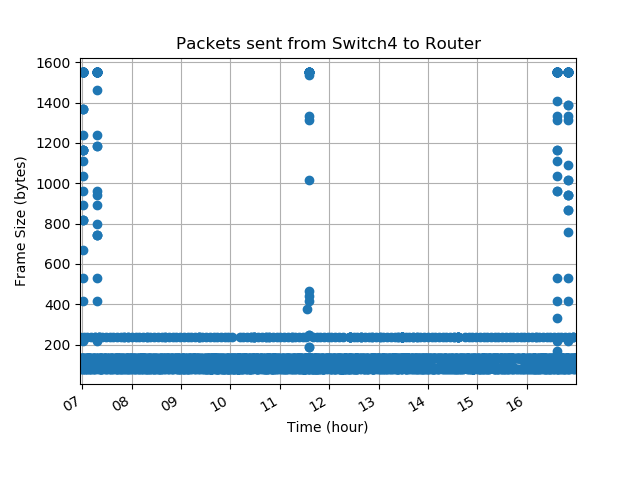
\includegraphics[width=\linewidth]{trngFromSwitch4}
			\caption{}
		\end{subfigure}
		\begin{subfigure}{.485\textwidth}
			\centering
			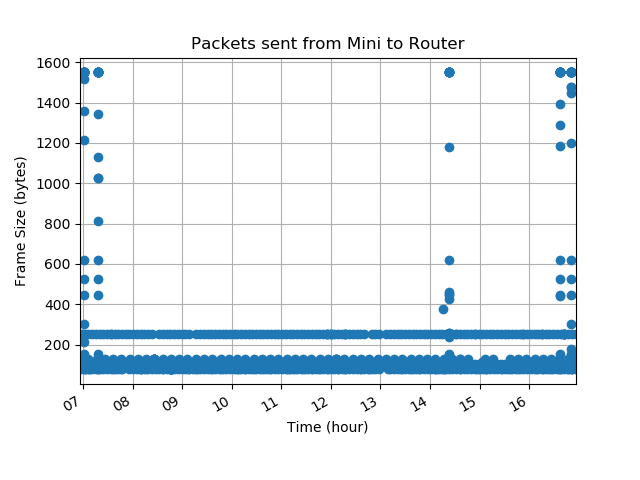
\includegraphics[width=\linewidth]{trngFromMini}
			\caption{}
		\end{subfigure}%
		\begin{subfigure}{.485\textwidth}
			\centering
			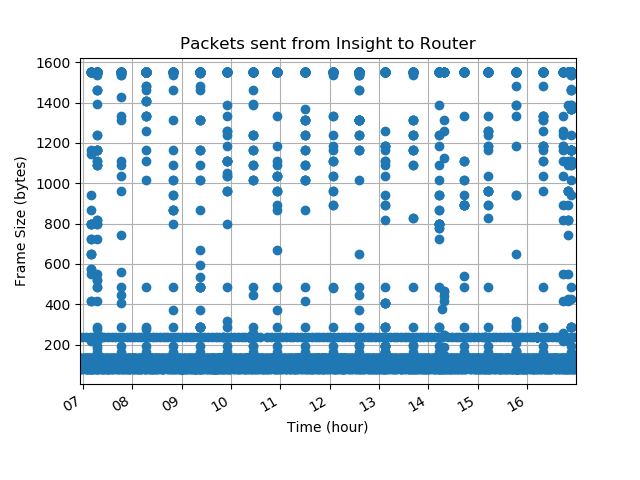
\includegraphics[width=\linewidth]{trngFromInsight}
			\caption{}
		\end{subfigure}
		\caption{Training plots of packets sent from device to the router}
		\label{fig:TrainingFromDevice}
	\end{figure}
}

\newcommand{\figClassificationToNetcam}{
	\begin{figure}[H]
		\begin{center}
			\makebox[\textwidth][c]{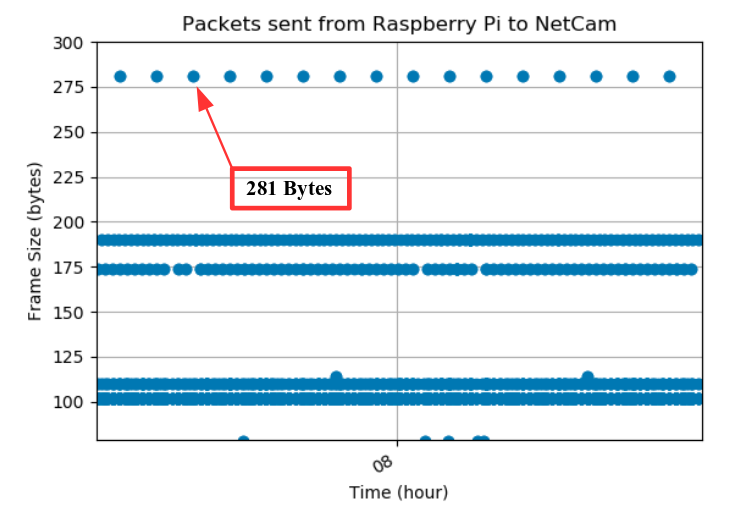
\includegraphics[width=5in]{classificationToNetcam}}
			\caption{Figure~\ref{fig:TrainingToDevice}(b) zoomed in on unique packet traffic used to classify camera devices}
			\label{fig:ClassificationToNetcam}
		\end{center}
		\vspace{-0.2 in}
	\end{figure}
}

\newcommand{\figClassificationToMotion}{
	\begin{figure}[H]
		\begin{center}
			\makebox[\textwidth][c]{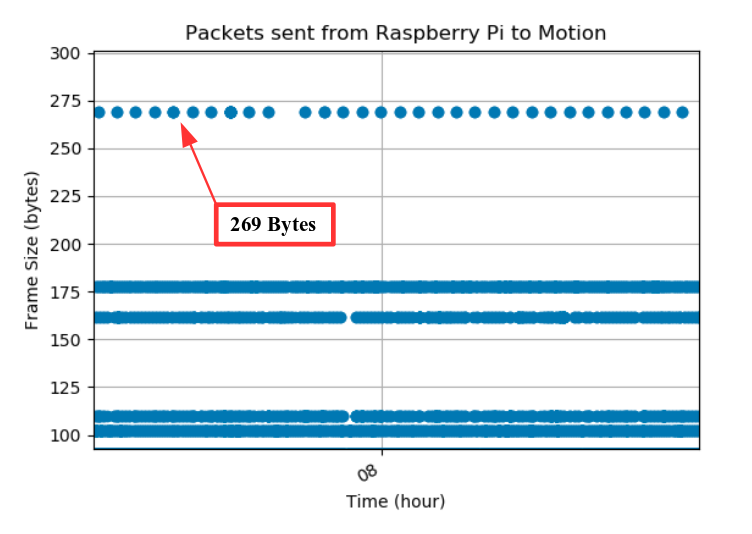
\includegraphics[width=5in]{classificationToMotion}}
			\caption{Figure~\ref{fig:TrainingToDevice}(a) zoomed in on unique packet traffic used to classify motion devices}
			\label{fig:ClassificationToMotion}
		\end{center}
		\vspace{-0.2 in}
	\end{figure}
}

\newcommand{\figClassificationToSwitch}{
	\begin{figure}[H]
		\begin{center}
			\makebox[\textwidth][c]{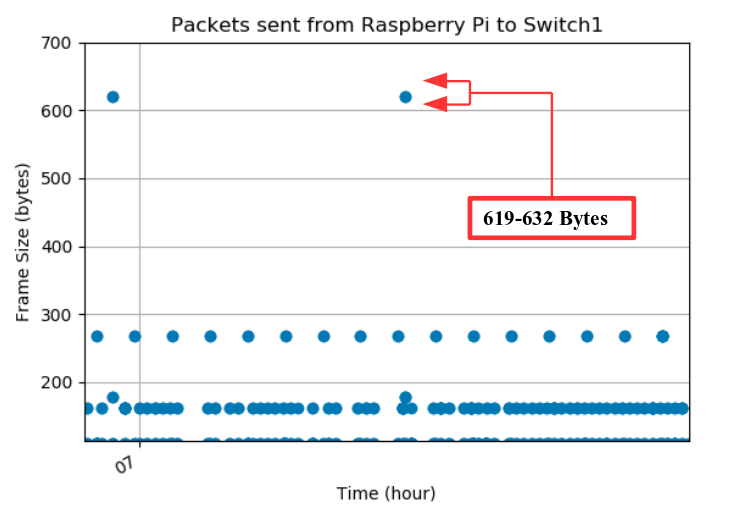
\includegraphics[width=5in]{classificationToSwitch}}
			\caption{Figure~\ref{fig:TrainingToDevice}(c) zoomed in on unique packet traffic used to classify outlet devices}
			\label{fig:ClassificationToSwitch}
		\end{center}
		\vspace{-0.2 in}
	\end{figure}
}

\newcommand{\figDeviceClassification}{
	\begin{figure}[H]
		\begin{center}
			\makebox[\textwidth][c]{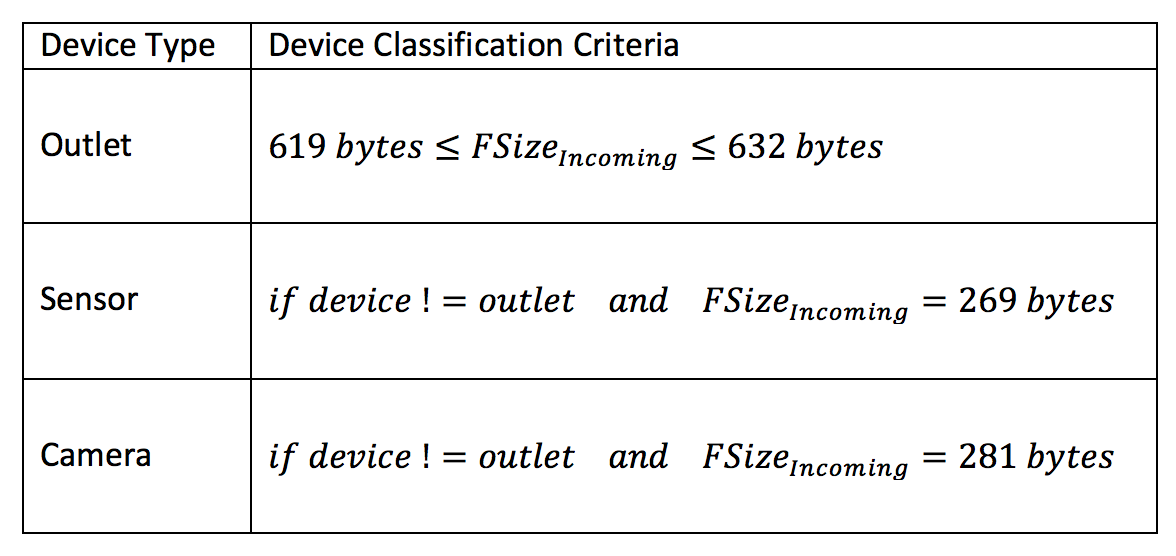
\includegraphics[height=2in]{deviceClassification}}
			\caption{Criteria used to classify devices}
			\label{fig:DeviceClassification}
		\end{center}
		\vspace{-0.2 in}
	\end{figure}
}

\newcommand{\figIdentificationToMini}{
	\begin{figure}[H]
		\begin{center}
			\makebox[\textwidth][c]{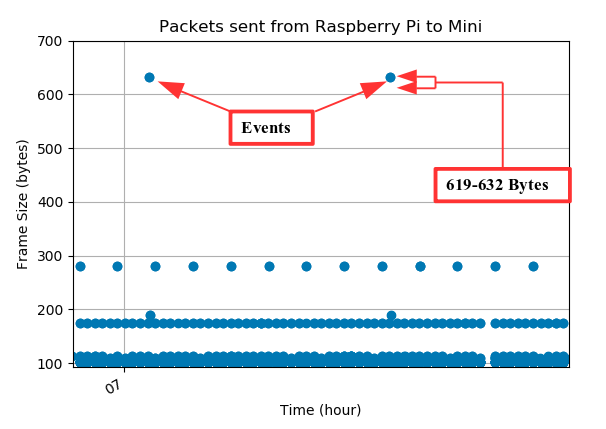
\includegraphics[width=5in]{identificationToMini}}
			\caption{Figure~\ref{fig:TrainingToDevice}(g) zoomed in on unique packet traffic used to identify outlet events}
			\label{fig:IdentificationToMini}
		\end{center}
		\vspace{-0.2 in}
	\end{figure}
}

\newcommand{\figIdentificationFromNetcam}{
	\begin{figure}[H]
		\begin{center}
			\makebox[\textwidth][c]{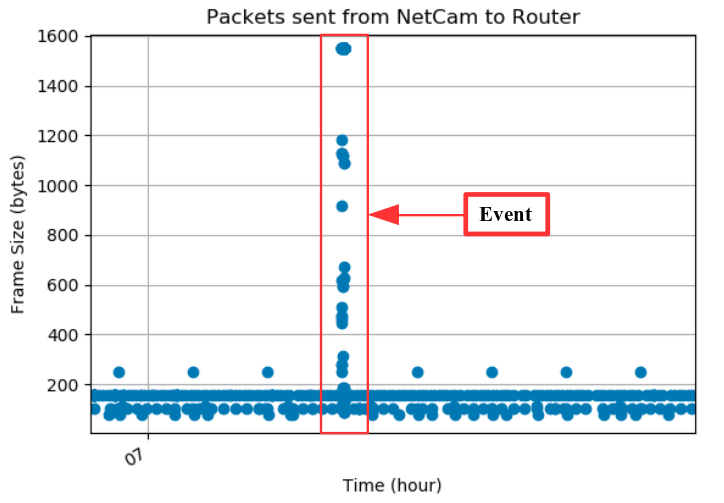
\includegraphics[width=5in]{identificationFromNetcam}}
			\caption{Figure~\ref{fig:TrainingFromDevice}(b) zoomed in on unique packet traffic used to identify camera events}
			\label{fig:IdentificationFromNetcam}
		\end{center}
		\vspace{-0.2 in}
	\end{figure}
}

\newcommand{\figIdentificationFromNetcamCum}{
	\begin{figure}[H]
		\begin{center}
			\makebox[\textwidth][c]{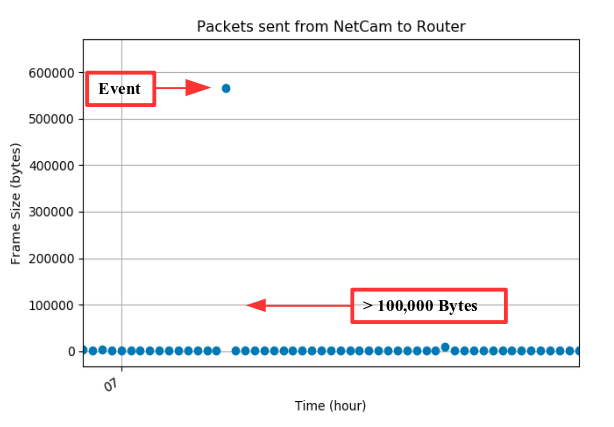
\includegraphics[width=5in]{identificationFromNetcamCum}}
			\caption{Figure~\ref{fig:TrainingFromDevice}(b) with one minute cumulative frame size zoomed in on unique packet traffic used to identify camera events}
			\label{fig:IdentificationFromNetcamCum}
		\end{center}
		\vspace{-0.2 in}
	\end{figure}
}

\newcommand{\figIdentificationFromMotion}{
	\begin{figure}[H]
		\begin{center}
			\makebox[\textwidth][c]{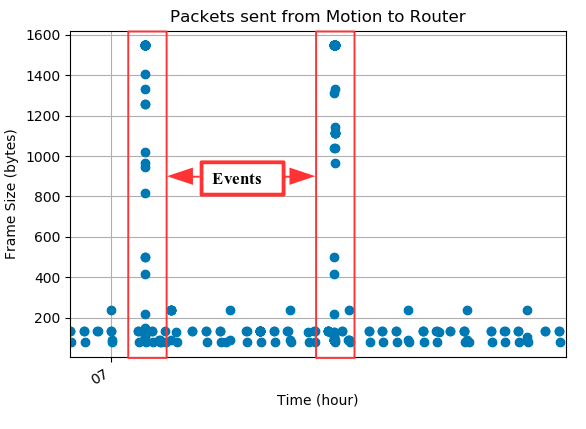
\includegraphics[width=5in]{identificationFromMotion}}
			\caption{Figure~\ref{fig:TrainingFromDevice}(a) zoomed in on unique packet traffic used to identify motion events}
			\label{fig:IdentificationFromMotion}
		\end{center}
		\vspace{-0.2 in}
	\end{figure}
}

\newcommand{\figIdentificationFromMotionCum}{
	\begin{figure}[H]
		\begin{center}
			\makebox[\textwidth][c]{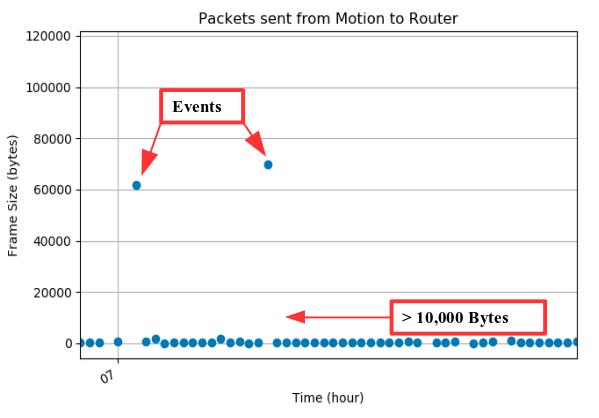
\includegraphics[width=5in]{identificationFromMotionCum}}
			\caption{Figure~\ref{fig:TrainingFromDevice}(a) with one minute cumulative frame size zoomed in on unique packet traffic used to identify motion events}
			\label{fig:IdentificationFromMotionCum}
		\end{center}
		\vspace{-0.2 in}
	\end{figure}
}

\newcommand{\figEventIdentification}{
	\begin{figure}[H]
		\begin{center}
			\makebox[\textwidth][c]{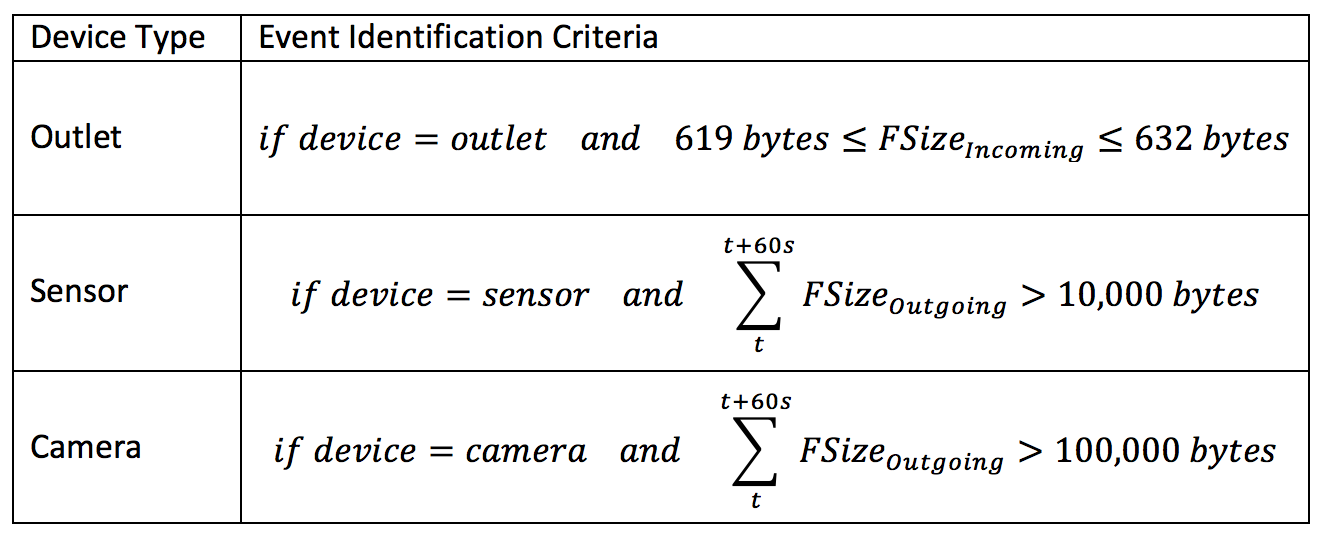
\includegraphics[height=2in]{eventIdentification}}
			\caption{Criteria used to identify events}
			\label{fig:EventIdentification}
		\end{center}
		\vspace{-0.2 in}
	\end{figure}
}

\newcommand{\figSubscribePacket}{
	\begin{figure}[H]
		\begin{center}
			\makebox[\textwidth][c]{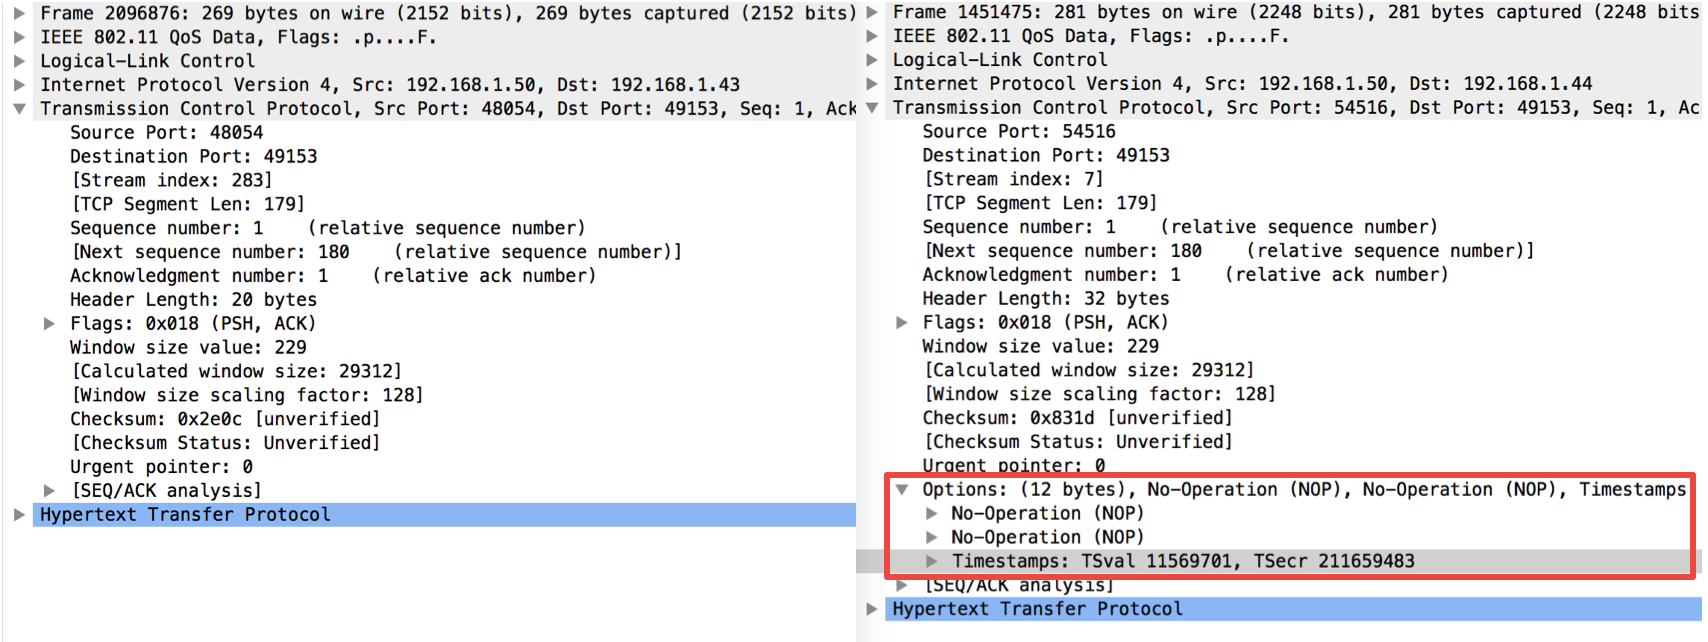
\includegraphics[width=\linewidth]{subscribePacket}}
			\caption{Decrypted \texttt{SUBSCRIBE} packets from Raspberry Pi to the NetCam and Motion devices depicting difference in frame length}
			\label{fig:SubscribePacket}
		\end{center}
		\vspace{-0.2 in}
	\end{figure}
}

\newcommand{\figPostPacket}{
	\begin{figure}[H]
		\begin{center}
			\makebox[\textwidth][c]{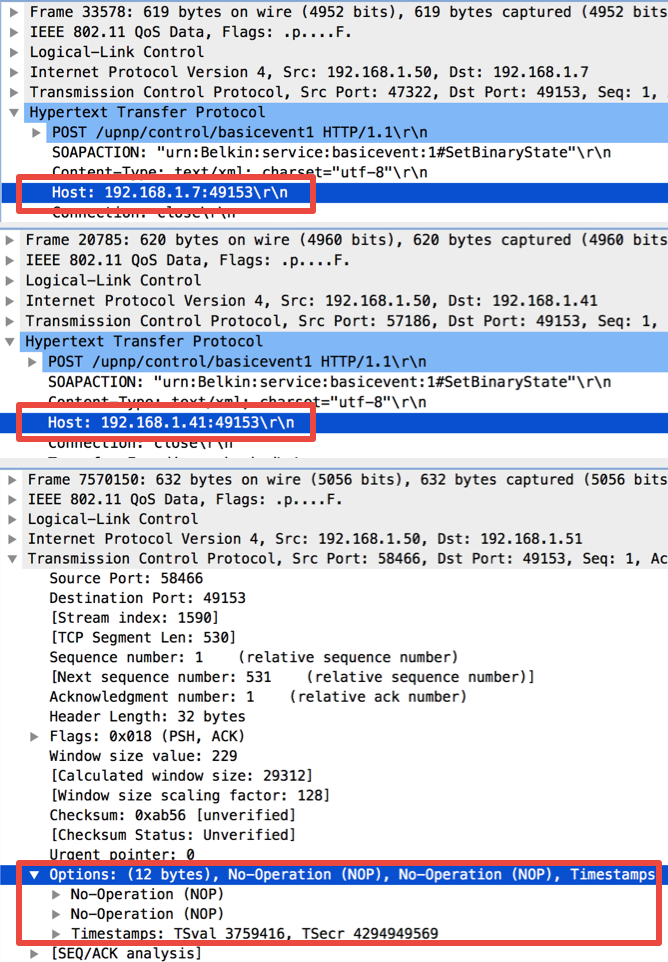
\includegraphics[width=.975\linewidth]{postPacket}}
			\caption{Decrypted \texttt{POST} packets from Raspberry Pi to the Switch4, Switch2, and Mini depicting differences in frame length}
			\label{fig:PostPacket}
		\end{center}
		\vspace{-0.2 in}
	\end{figure}
}

\newcommand{\figNetworkMap}{
	\begin{figure}[H]
		\begin{center}
			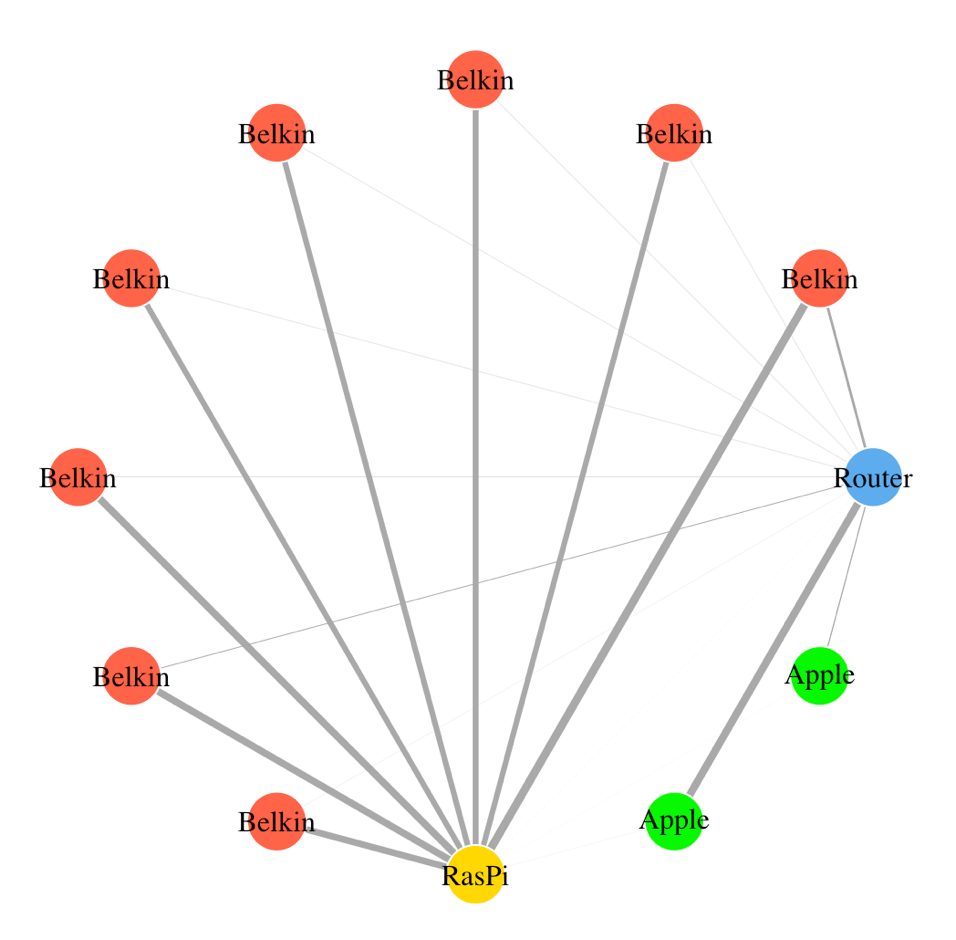
\includegraphics[width=5in]{networkMap}
			\caption{Network mapping of smart home architecture}
			\label{fig:NetworkMap}
		\end{center}
		\vspace{-0.2 in}
	\end{figure}
}

\newcommand{\figMiotlDiagram}{
	\begin{figure*}[h!]
		\begin{center}
			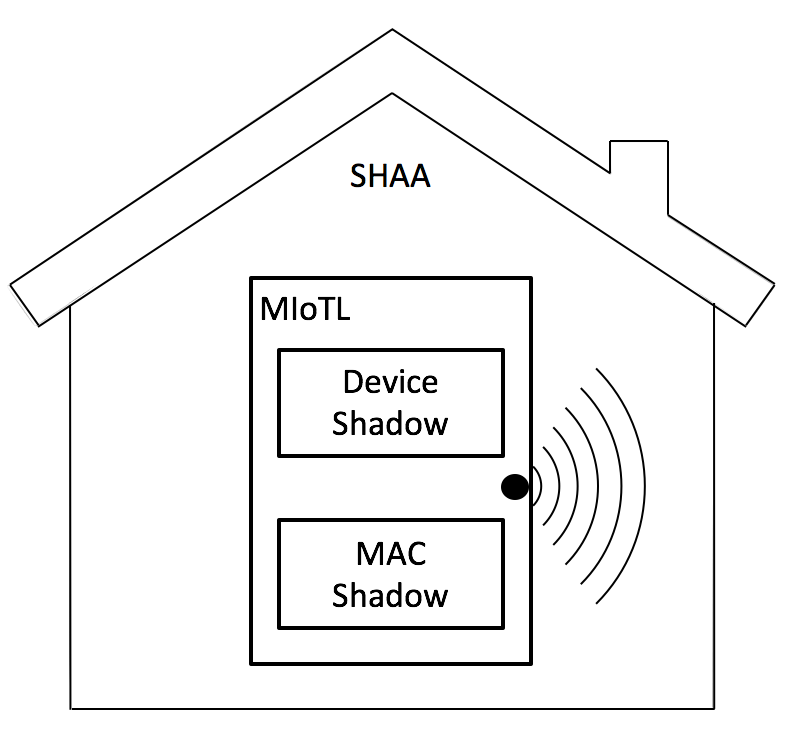
\includegraphics[width=3in]{miotlDiagram}
			\caption{Diagram of MIoTL tool components}
			\label{fig:MiotlDiagram}
		\end{center}
		\vspace{-0.2 in}
	\end{figure*}
}

\newcommand{\figSutCutDiagram}{
	\begin{figure*}[h!]
		\begin{center}
			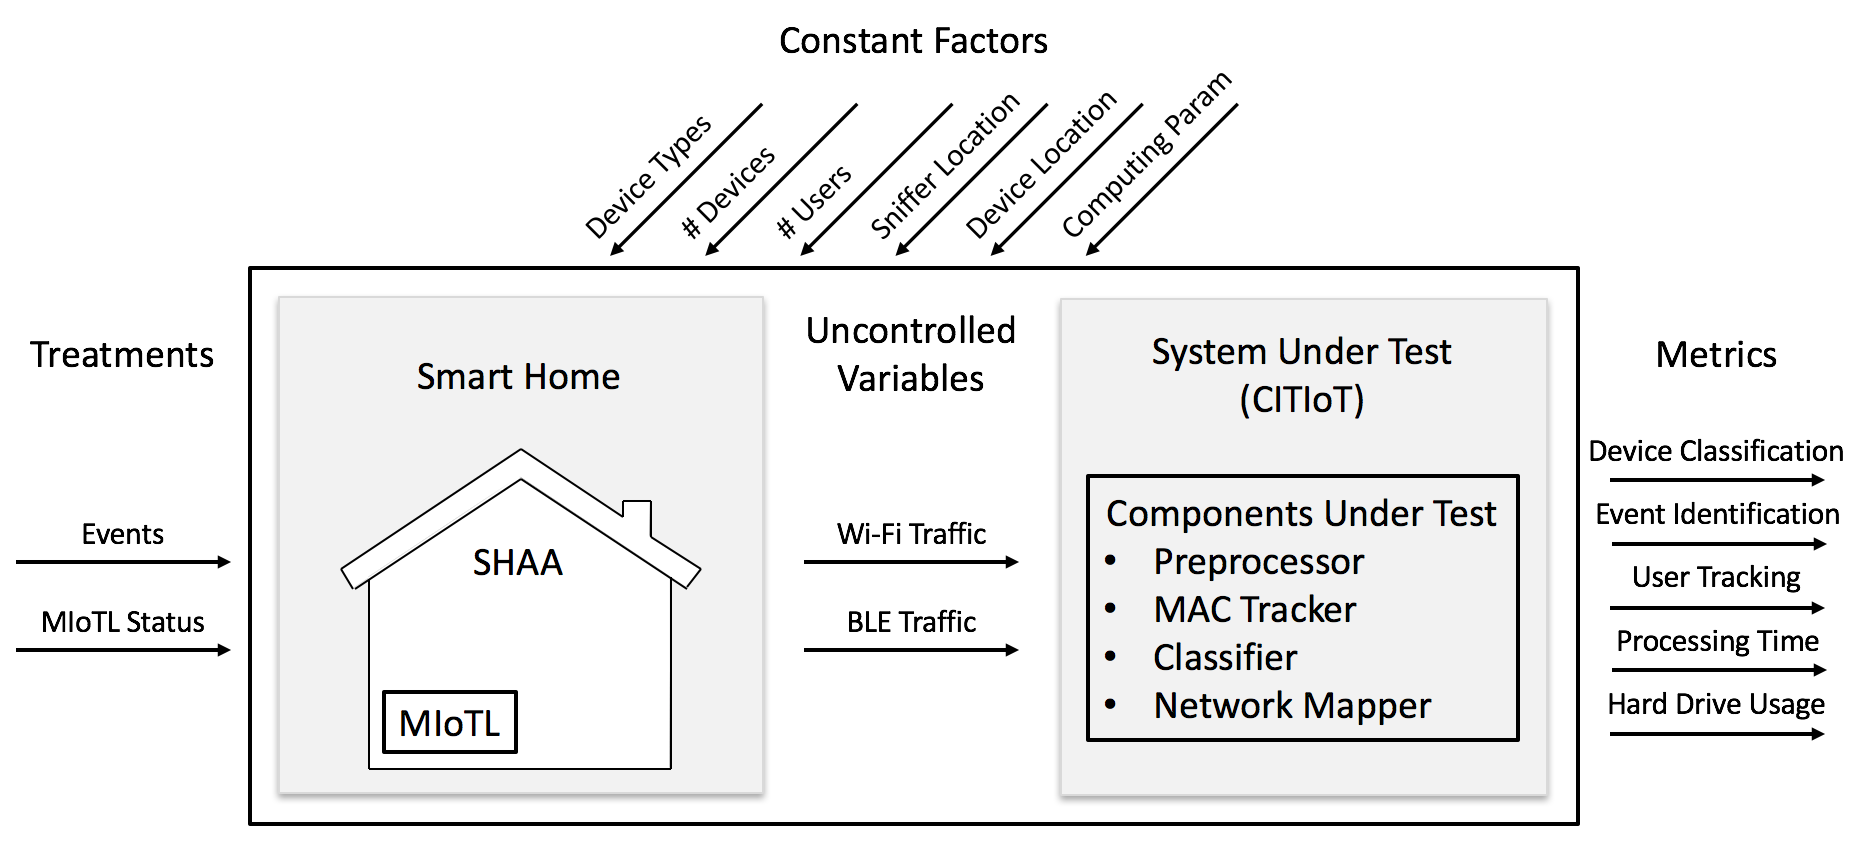
\includegraphics[width=\linewidth]{sutCutDiagram}
			\caption{System Under Test (SUT) and Component Under Test (CUT) diagram}
			\label{fig:SutCutDiagram}
		\end{center}
		\vspace{-0.2 in}
	\end{figure*}
}

\newcommand{\figShaaExperimentDiagram}{
	\begin{figure*}[h!]
		\begin{center}
			\includegraphics[width=\linewidth]{shaaExperimentDiagram}
			\caption{Approximate layout of devices within \ac{SHAA} for experimentation (not to scale)}
			\label{fig:ShaaExperimentDiagram}
		\end{center}
		\vspace{-0.2 in}
	\end{figure*}
}

\newcommand{\figSnifferExperimentSetup}{
	\begin{figure*}[h!]
		\begin{center}
			\includegraphics[width=\linewidth]{snifferExperimentSetup}
			\caption{Layout of sniffer antennae for experimentation}
			\label{fig:SnifferExperimentSetup}
		\end{center}
		\vspace{-0.2 in}
	\end{figure*}
}

\newcommand{\figDataCollectionFramework}{
	\begin{figure}[h!]
		\begin{center}
			\includegraphics[width=\linewidth, height = 5cm]{hostMachine}
			\caption{Data Collection Framework}
			\label{fig:DataCollectionFramework}
		\end{center}
		\vspace{-0.2 in}
	\end{figure}
}

\newcommand{\figSampleResults}{
\begin{figure}[H]
	\begin{center}
		\includegraphics[width=\linewidth]{sampleResults}
		\caption{Example graph comparing CITIoT events with actual events}
		\label{fig:SampleResults}
	\end{center}
	\vspace{-0.2 in}
\end{figure}
}

\newcommand{\figCitiot}{
	\begin{figure}[H]
		\begin{center}
			\makebox[\textwidth][c]{\includegraphics[width=5in]{citiot}}
			\caption{CITIoT Architecture}
			\label{fig:Citiot}
		\end{center}
		\vspace{-0.2 in}
	\end{figure}
}

\newcommand{\figReconScanning}{
	\begin{figure}[H]
		\begin{center}
			\makebox[\textwidth][c]{\includegraphics[width=5in]{reconScanning}}
			\caption{Scanning command along with output.}
			\label{fig:ReconScanning}
		\end{center}
		\vspace{-0.2 in}
	\end{figure}
}

\newcommand{\figNetworkMapping}{
	\begin{figure}[tbp]
		\begin{center}
			\includegraphics[width=3in, height=7cm]{networkMapping}
			\caption{Network mapping of smart home architecture; thicker lines mean stronger correlation between devices.}
			\label{fig:NetworkMapping}
		\end{center}
		\vspace{-0.2 in}
	\end{figure}
}

\newcommand{\figMethodologyOverview}{
	\begin{figure}[H]
		\begin{center}
			\makebox[\textwidth][c]{\includegraphics[width=6in]{methodologyOverview}}
			\caption{Overall scenario setup.}
			\label{fig:MethodologyOverview}
		\end{center}
		\vspace{-0.2 in}
	\end{figure}
}

\newcommand{\figDeviceId}{
	\begin{figure}[H]
	\centering
		\begin{minipage}{.5\textwidth}
			\centering
			\includegraphics[width=1\linewidth]{deviceIdOutlet}
			\caption{Outlet device.}
			\label{fig:DeviceIdOutlet}
		\end{minipage}%
		\begin{minipage}{.5\textwidth}
			\centering
			\includegraphics[width=1\linewidth]{deviceIdSensor}
			\caption{Sensor device.}
			\label{fig:DeviceIdSensor}
		\end{minipage}
		\begin{minipage}{.5\textwidth}
			\centering
			\includegraphics[width=1\linewidth]{deviceIdCamera}
			\caption{Camera device.}
			\label{fig:DeviceIdCamera}
		\end{minipage}
	\end{figure}
}


\newcommand{\figExamplePlotOne}{
	\begin{figure}[H]
		\begin{center}
			\makebox[\textwidth][c]{\includegraphics[width=4.5in]{examplePlot1}}
			\caption{Example Plot One: Event Identification}
			\label{fig:ExamplePlotOne}
		\end{center}
		\vspace{-0.2 in}
	\end{figure}
}

\newcommand{\figExamplePlotTwo}{
	\begin{figure}[H]
		\begin{center}
			\makebox[\textwidth][c]{\includegraphics[width=4.5in]{examplePlot2}}
			\caption{Example Plot Two: Time User is Home}
			\label{fig:ExamplePlotTwo}
		\end{center}
		\vspace{-0.2 in}
		\end{figure}
}

\newcommand{\figafitStyle}{\begin{figure}[tbp]
 \begin{center}
    \includegraphics[width=6in]{myFirstLaTeXafit}
     \caption{Recompile using afitThesis.sty, the AFIT
     thesis style file.}
     \label{fig:afitStyle}
 \end{center}
\end{figure}
}


\newcommand{\figtitlePage}{\begin{figure}[tbp]
 \begin{center}
    \includegraphics[width=6in]{titlePage}
     \caption{Enter student data in titlePage.tex to customize the
     document's first pages.}
     \label{fig:titlePage}
 \end{center}
\end{figure}
}

\newcommand{\figmyFlypage}{\begin{figure}[tbp]
 \begin{center}
    \includegraphics[width=6in]{myFlypage}
     \caption{Here we have compiled the first four page of a thesis.}
     \label{fig:myFlypage}
 \end{center}
\end{figure}
}

\newcommand{\figmyFirstAbstract}{\begin{figure}[tbp]
 \begin{center}
    \includegraphics[width=6in]{myFirstAbstract}
     \caption{Add an abstract to the front matter of your thesis.}
     \label{fig:myFirstAbstract}
 \end{center}
\end{figure}
}

\newcommand{\figmyFigures}{\begin{figure}[tbp]
 \begin{center}
    \includegraphics[width=5in]{myFigures}
     \caption{Consider defining all your figures in one file.}
     \label{fig:myFigures}
 \end{center}
\end{figure}
}


\newcommand{\figmyFirstFigures}{\begin{figure}[tbp]
 \begin{center}
    \includegraphics[width=6in]{myFirstFigures}
     \caption{Add figures in the main matter of your document; fill in
     the document around your graphics.}
     \label{fig:myFirstFigures}
 \end{center}
\end{figure}
}

\newcommand{\figmyFirstBibTeX}{\begin{figure}[tbp]
 \begin{center}
    \includegraphics[width=6in]{myFirstBibTeX}
     \caption{Add your bibliography.}
     \label{fig:myFirstBibTeX}
 \end{center}
\end{figure}
}



